\documentclass[11pt,a4paper]{article}

\usepackage[utf8]{inputenc}
\usepackage[T1]{fontenc}
\usepackage{lmodern}
\usepackage{amsmath,amssymb,amsfonts,amsthm}
\usepackage{graphicx}
\usepackage{booktabs}
\usepackage{microtype}
\usepackage{hyperref}
\usepackage[numbers,sort&compress]{natbib}
\usepackage{geometry}
\usepackage{xcolor}
\usepackage{caption}
\usepackage{subcaption}

\geometry{
  top=2.5cm,
  bottom=2.5cm,
  left=2.5cm,
  right=2.5cm
}

\hypersetup{
  colorlinks=true,
  linkcolor=blue!70!black,
  citecolor=blue!70!black,
  urlcolor=blue!70!black,
  pdfauthor={Pavan B. Govindaraju},
  pdftitle={On the Non-Negativity of Longitudinal Velocity Autocorrelations in Homogeneous Isotropic Turbulence: Kinematic Constraints, Convexity, and Spectral Broadening}
}

\newtheorem{theorem}{Theorem}
\newtheorem{lemma}[theorem]{Lemma}
\newtheorem{proposition}[theorem]{Proposition}
\newtheorem{corollary}[theorem]{Corollary}
\theoremstyle{definition}
\newtheorem{definition}{Definition}
\newtheorem{remark}{Remark}

\title{\textbf{\Large On the Non-Negativity of Longitudinal Velocity Autocorrelations in Homogeneous Isotropic Turbulence: Kinematic Constraints, Convexity, and Spectral Broadening}}

\author{
  \textbf{Pavan B. Govindaraju}\thanks{Email: \href{mailto:pavan@splitfxm.com}{pavan@splitfxm.com}} \\
  \textit{SplitFXM}
}

\date{\today}

\begin{document}

\maketitle

\begin{abstract}
A fundamental question in the statistical theory of homogeneous isotropic turbulence is whether the longitudinal two-point velocity autocorrelation function, $f(r)$, must remain strictly non-negative for all spatial separations $r$ from first principles of kinematic realizability. While the lateral correlation $g(r)$ is kinematically constrained by incompressibility to cross zero and exhibit a negative loop ($\int_0^\infty r g(r)\,dr = 0$), the sign behavior of $f(r)$ has remained subtle. In this paper, we resolve the non-negativity question. First, we demonstrate that classical positive-definiteness arguments based on Bochner's and Schoenberg's theorems structurally fail to enforce pointwise positivity because the underlying spherical projection kernels in $\mathbb{R}^3$ are intrinsically sign-changing. Second, by mapping the problem onto the one-dimensional longitudinal energy spectrum $E_{11}(k_1)$ via the Wiener--Khinchin cosine transform, we prove that $E_{11}(k_1)$ is unconditionally monotonically decreasing for \emph{any} admissible three-dimensional energy spectrum $E(k) \ge 0$. Third, applying P\'olya's criterion for characteristic functions, we establish that convexity of $E_{11}(k_1)$ is a rigorous sufficient condition for $f(r) \ge 0$ for all $r$. We prove that while pure Kolmogorov $-5/3$ scaling is strictly convex, any physically realizable, Batchelor-consistent spectrum ($E(k) \sim k^4$ as $k \to 0$) is necessarily concave in a finite infrared neighborhood near $k_1 = 0$. For mature, broadband spectra (such as the von K\'arm\'an--Pao model), high-precision infinite-limit quadrature proves that the convex inertial bulk dominates, yielding strictly non-negative correlation tails and revealing previous negative dips in the literature to be numerical artifacts of discrete Fourier transforms. Finally, we construct a smooth, divergence-free, finite-energy, Batchelor-consistent narrowband counterexample that constitutes valid initial data for the Navier--Stokes equations and produces a pronounced, genuine negative loop ($\min_r f(r) \approx -0.083$). We show that this mathematical transition matches the experimental emergence and subsequent disappearance of negative loops in grid-generated turbulence, where nonlinear triad cascade broadens the spectrum over an eddy turnover time.
\end{abstract}

\vspace{0.5em}
\noindent\textbf{Keywords:} Homogeneous isotropic turbulence, velocity autocorrelations, P\'olya's criterion, Bochner's theorem, spectral broadening, grid turbulence.

\section{Introduction}
\label{sec:intro}

The statistical description of homogeneous isotropic turbulence (HIT), initiated by Taylor \cite{Taylor1935} and formalized by von K\'arm\'an \& Howarth \cite{vonKarmanHowarth1938} and Robertson \cite{Robertson1940}, rests upon the two-point velocity correlation tensor
\begin{equation}
R_{ij}(\mathbf{r}, t) = \langle u_i(\mathbf{x}, t) u_j(\mathbf{x} + \mathbf{r}, t) \rangle,
\label{eq:Rij_def}
\end{equation}
where $\mathbf{u}(\mathbf{x}, t)$ is the divergence-free fluctuating velocity field and angle brackets denote an ensemble average. Under spatial isotropy and reflectional invariance, the nine components of $R_{ij}(\mathbf{r}, t)$ collapse entirely onto two scalar correlation coefficients: the longitudinal autocorrelation function $f(r, t)$ and the lateral (transverse) autocorrelation function $g(r, t)$, defined by
\begin{equation}
R_{ij}(\mathbf{r}, t) = u'^2 \left[ g(r, t)\,\delta_{ij} + \big(f(r, t) - g(r, t)\big)\,\frac{r_i r_j}{r^2} \right],
\label{eq:Rij_isotropic}
\end{equation}
with $r = |\mathbf{r}|$, $u'(t) = \langle u_1^2 \rangle^{1/2}$, and normalized such that $f(0, t) = g(0, t) = 1$.

Incompressible mass conservation ($\nabla \cdot \mathbf{u} = 0$) enforces the well-known differential kinematic relation
\begin{equation}
g(r, t) = f(r, t) + \frac{r}{2} \frac{\partial f(r, t)}{\partial r} = \frac{1}{2r} \frac{\partial}{\partial r}\big(r^2 f(r, t)\big).
\label{eq:continuity_fg}
\end{equation}
Integrating Eq.~\eqref{eq:continuity_fg} over all separation distances yields an exact integral constraint for the lateral correlation:
\begin{equation}
\int_0^\infty r\,g(r, t)\,dr = \frac{1}{2} \Big[ r^2 f(r, t) \Big]_0^\infty = 0,
\label{eq:g_zero_integral}
\end{equation}
provided that $r^2 f(r, t) \to 0$ as $r \to \infty$. Because $g(0, t) = 1 > 0$, Eq.~\eqref{eq:g_zero_integral} strictly forces $g(r, t)$ to cross zero and attain negative values over a finite interval of separations---a phenomenon ubiquitously referred to as the \emph{transverse negative loop} \cite{Batchelor1953, MoninYaglom1975, Pope2000, Davidson2015}.

In contrast, no such kinematic integral constraint exists for the longitudinal correlation $f(r, t)$. The longitudinal integral scale,
\begin{equation}
L(t) = \int_0^\infty f(r, t)\,dr,
\label{eq:integral_scale}
\end{equation}
is strictly positive for all physically realizable turbulent fields. In textbooks and classical closure theories, $f(r)$ is frequently depicted as a strictly non-negative, monotonically decreasing function \cite{Pope2000, Frisch1995, Sedov1944, Ran2009}. However, this raises a foundational question:
\begin{quote}
\emph{Is the longitudinal velocity autocorrelation function $f(r)$ non-negative for all spatial separations $r$ from first principles of kinematic realizability, or can $f(r)$ become negative?}
\end{quote}

This question has persisted across both theoretical mechanics and experimental measurements. Early grid-turbulence experiments by Stewart \& Townsend \cite{StewartTownsend1951} and Frenkiel et al. \cite{FrenkielKlebanoffHuang1979} documented small but persistent negative loops in measured spatial longitudinal correlation functions near turbulence-generating grids. Furthermore, in their seminal investigations of space-time and Eulerian velocity correlations in grid turbulence, Comte-Bellot \& Corrsin \cite{ComteBellotCorrsin1971} demonstrated that narrow-band filtered velocity signals exhibit pronounced oscillatory negative loops, whereas full-band signals decay smoothly, while also highlighting how AC-coupling and finite domain sizes force measured integral scales to vanish experimentally. Yet, it has remained unsettled whether such spatial excursions are mere measurement noise, instrumentation artifacts, or genuine physical consequences of Navier--Stokes dynamics and kinematic realizability.

In this work, we provide a complete mathematical and physical resolution to this question:
\begin{enumerate}
\item We show that positive definiteness in $\mathbb{R}^3$ via Bochner's and Schoenberg's theorems \cite{Bochner1959, Schoenberg1938} cannot establish $f(r) \ge 0$ because the associated projection kernels oscillate and change sign.
\item By analyzing the one-dimensional longitudinal energy spectrum $E_{11}(k_1)$, we prove that $E_{11}(k_1)$ is \emph{unconditionally monotonically decreasing} for every realizable 3D spectrum $E(k) \ge 0$, and we establish via P\'olya's criterion \cite{Polya1918, Polya1949} that convexity of $E_{11}(k_1)$ is a rigorous sufficient condition for $f(r) \ge 0$.
\item We prove that every physically admissible, Batchelor-consistent spectrum ($E(k) \sim k^4$ as $k \to 0$) is necessarily concave in a finite neighborhood of the origin ($k_1 \to 0$), so P\'olya's sufficient condition is never strictly satisfied in a global sense.
\item For mature broadband spectra (e.g., von K\'arm\'an--Pao), high-precision infinite-limit quadrature demonstrates that the convex inertial bulk dominates the cosine transform, ensuring $f(r) \ge 0$ everywhere and identifying previous negative dips in the literature as discrete Fourier transform (FFT) aliasing artifacts.
\item We construct an admissible, smooth, divergence-free, finite-energy narrowband spectrum satisfying Batchelor's infrared constraint that yields a pronounced, provable negative loop ($\min_r f(r) \approx -0.083$). This state is a legitimate Navier--Stokes initial condition whose evolution is guaranteed by classical local existence theorems \cite{Leray1934, FujitaKato1964}, directly matching experimental observations in near-grid turbulence before nonlinear triad interactions broaden the spectrum.
\end{enumerate}

\section{Kinematics and the Failure of Naive Positive Definiteness}
\label{sec:bochner_failure}

\subsection{Invariant Tensor Theory and Derivation of the Isotropic Form of \texorpdfstring{$R_{ij}(\mathbf{r})$}{Rij(r)}}
\label{subsec:rij_derivation}

We begin by establishing from first principles why the two-point velocity correlation tensor $R_{ij}(\mathbf{r}) = \langle u_i(\mathbf{x}) u_j(\mathbf{x}+\mathbf{r}) \rangle$ in homogeneous isotropic turbulence depends entirely on just two scalar correlation functions, $f(r)$ and $g(r)$.

\paragraph{1. Homogeneity (Translational Invariance):}
Statistical homogeneity implies that the correlation depends only on the separation vector $\mathbf{r} = \mathbf{x}' - \mathbf{x}$ and is independent of the absolute spatial location $\mathbf{x}$. Shifting the origin of averaging by $-\mathbf{r}$ yields
\begin{equation}
R_{ij}(-\mathbf{r}) = \langle u_i(\mathbf{x}) u_j(\mathbf{x}-\mathbf{r}) \rangle = \langle u_i(\mathbf{x}+\mathbf{r}) u_j(\mathbf{x}) \rangle = \langle u_j(\mathbf{x}) u_i(\mathbf{x}+\mathbf{r}) \rangle = R_{ji}(\mathbf{r}).
\label{eq:Rij_homogeneity_sym}
\end{equation}

\paragraph{2. Isotropy (Rotational Invariance):}
Statistical isotropy requires that under any coordinate rotation $Q \in \mathrm{SO}(3)$ (where $Q_{ik} Q_{jk} = \delta_{ij}$ and $\det Q = +1$), the correlation tensor transforms as an isotropic second-order tensor field:
\begin{equation}
R_{ij}(Q\mathbf{r}) = Q_{im} Q_{jn} R_{mn}(\mathbf{r}).
\label{eq:Rij_rotation}
\end{equation}
By the invariant tensor representation theorem for vector-valued isotropic functions (Robertson \cite{Robertson1940}; Batchelor \cite{Batchelor1953}), any second-order tensor constructed from a single vector argument $\mathbf{r}$ and the fundamental isotropic tensors ($\delta_{ij}$ and the Levi-Civita permutation symbol $\epsilon_{ijk}$) must be a linear combination of the three fundamental isotropic second-order forms:
\begin{equation}
R_{ij}(\mathbf{r}) = A(r)\,\delta_{ij} + B(r)\,r_i r_j + C(r)\,\epsilon_{ijk} r_k,
\label{eq:Rij_general_isotropic}
\end{equation}
where $r = |\mathbf{r}| = \sqrt{r_k r_k}$ is the sole scalar invariant, and $A(r), B(r), C(r)$ are scalar functions of $r$.

\paragraph{3. Reflection Invariance (Parity / Zero Mean Helicity):}
Under a spatial reflection through the origin ($\mathbf{r} \to -\mathbf{r}$, $\mathbf{u} \to -\mathbf{u}$), a true (polar) velocity vector satisfies $\langle u_i(-\mathbf{x}) u_j(-\mathbf{x}-\mathbf{r}) \rangle = R_{ij}(\mathbf{r})$. Applying this to Eq.~\eqref{eq:Rij_general_isotropic}:
\begin{equation}
R_{ij}(-\mathbf{r}) = A(r)\,\delta_{ij} + B(r)\,(-r_i)(-r_j) + C(r)\,\epsilon_{ijk}(-r_k) = A(r)\,\delta_{ij} + B(r)\,r_i r_j - C(r)\,\epsilon_{ijk} r_k.
\end{equation}
Combining this with homogeneity ($R_{ij}(-\mathbf{r}) = R_{ji}(\mathbf{r}) = A(r)\delta_{ij} + B(r)r_i r_j - C(r)\epsilon_{ijk} r_k$) and symmetry requires
\begin{equation}
C(r) \equiv 0.
\end{equation}
Physically, $C(r)$ represents turbulent helicity ($\langle \mathbf{u} \cdot (\nabla \times \mathbf{u}) \rangle$), which identically vanishes for reflectionally invariant isotropic turbulence. Hence, $R_{ij}(\mathbf{r})$ is strictly symmetric:
\begin{equation}
R_{ij}(\mathbf{r}) = A(r)\,\delta_{ij} + B(r)\,r_i r_j.
\label{eq:Rij_symmetric}
\end{equation}

\paragraph{4. Identification with Longitudinal and Lateral Correlations:}
To determine $A(r)$ and $B(r)$ physically, align the coordinate system such that the separation vector lies along the $x_1$-axis: $\mathbf{r} = (r, 0, 0)$.
\begin{itemize}
\item The \emph{longitudinal autocorrelation} is the correlation of the velocity component parallel to the separation vector:
\begin{equation}
R_{11}(r \mathbf{e}_1) = \langle u_1(\mathbf{x}) u_1(\mathbf{x} + r\mathbf{e}_1) \rangle \equiv u'^2 f(r).
\label{eq:f_def_parallel}
\end{equation}
Evaluating Eq.~\eqref{eq:Rij_symmetric} for $i=j=1$ gives
\begin{equation}
R_{11}(r \mathbf{e}_1) = A(r) + B(r)\,r^2 = u'^2 f(r).
\label{eq:match_longitudinal}
\end{equation}
\item The \emph{lateral (transverse) autocorrelation} is the correlation of a velocity component perpendicular to the separation vector (e.g., $u_2$ or $u_3$):
\begin{equation}
R_{22}(r \mathbf{e}_1) = \langle u_2(\mathbf{x}) u_2(\mathbf{x} + r\mathbf{e}_1) \rangle \equiv u'^2 g(r).
\label{eq:g_def_transverse}
\end{equation}
Evaluating Eq.~\eqref{eq:Rij_symmetric} for $i=j=2$ gives
\begin{equation}
R_{22}(r \mathbf{e}_1) = A(r) = u'^2 g(r).
\label{eq:match_lateral}
\end{equation}
\end{itemize}
Substituting $A(r) = u'^2 g(r)$ into Eq.~\eqref{eq:match_longitudinal} yields
\begin{equation}
B(r)\,r^2 = u'^2 \big(f(r) - g(r)\big) \implies B(r) = u'^2\,\frac{f(r) - g(r)}{r^2}.
\label{eq:solve_B}
\end{equation}
Substituting $A(r)$ and $B(r)$ back into Eq.~\eqref{eq:Rij_symmetric} gives the canonical tensorial form of von K\'arm\'an \& Howarth \cite{vonKarmanHowarth1938}:
\begin{equation}
R_{ij}(\mathbf{r}) = u'^2 \left[ g(r)\,\delta_{ij} + \big(f(r) - g(r)\big)\,\frac{r_i r_j}{r^2} \right].
\label{eq:Rij_canonical_proven}
\end{equation}
Thus, any homogeneous, isotropic, reflection-symmetric second-order velocity correlation tensor in three dimensions is uniquely and completely determined by the two scalar functions $f(r)$ and $g(r)$.

\subsection{Spectral Tensors and Kinematic Realizability}

The spatial Fourier transform of the two-point velocity correlation tensor $R_{ij}(\mathbf{r})$ is the velocity spectrum tensor $\Phi_{ij}(\mathbf{k})$:
\begin{equation}
R_{ij}(\mathbf{r}) = \iiint_{\mathbb{R}^3} \Phi_{ij}(\mathbf{k})\,e^{i \mathbf{k} \cdot \mathbf{r}}\,d\mathbf{k}, \qquad
\Phi_{ij}(\mathbf{k}) = \frac{1}{(2\pi)^3} \iiint_{\mathbb{R}^3} R_{ij}(\mathbf{r})\,e^{-i \mathbf{k} \cdot \mathbf{r}}\,d\mathbf{r}.
\label{eq:spectral_tensor_pair}
\end{equation}
Incompressible continuity ($\nabla \cdot \mathbf{u} = 0$) requires $k_i \Phi_{ij}(\mathbf{k}) = k_j \Phi_{ij}(\mathbf{k}) = 0$. For an isotropic, reflection-symmetric field, the spectrum tensor takes the unique form \cite{Batchelor1953, Pope2000}
\begin{equation}
\Phi_{ij}(\mathbf{k}) = \frac{E(k)}{4\pi k^4} \left( k^2 \delta_{ij} - k_i k_j \right),
\label{eq:Phi_ij_isotropic}
\end{equation}
where $k = |\mathbf{k}|$ is the magnitude of the wavevector, and $E(k)$ is the three-dimensional turbulent kinetic energy spectrum, normalized such that
\begin{equation}
\frac{3}{2} u'^2 = \frac{1}{2} \langle u_i u_i \rangle = \int_0^\infty E(k)\,dk.
\label{eq:TKE_norm}
\end{equation}
Kinematic realizability dictates that for any complex vector field $a_i(\mathbf{k})$, the quadratic form $a_i^*(\mathbf{k}) \Phi_{ij}(\mathbf{k}) a_j(\mathbf{k}) \ge 0$, which is equivalent to requiring that the energy spectrum satisfies
\begin{equation}
E(k) \ge 0 \quad \text{for all } k \in [0, \infty).
\label{eq:realizability_Ek}
\end{equation}

\subsection{Schoenberg's Theorem and Radial Projection Kernels}

A natural conjecture is whether Bochner's theorem \cite{Bochner1959}---which guarantees that any positive-definite function on $\mathbb{R}^n$ is the Fourier transform of a non-negative finite Borel measure---implies that the spatial correlation functions $f(r)$ and $g(r)$ are non-negative.

By Schoenberg's classical representation theorem \cite{Schoenberg1938}, an isotropic (radial) scalar function $\psi(r)$ on $\mathbb{R}^n$ is positive definite if and only if it admits the integral representation
\begin{equation}
\psi(r) = \int_0^\infty \Omega_n(kr)\,d\nu(k), \qquad \nu \ge 0,
\label{eq:schoenberg_rep}
\end{equation}
where the radial projection kernel $\Omega_n(x)$ is given in terms of the Bessel function of the first kind:
\begin{equation}
\Omega_n(x) = \Gamma\left(\frac{n}{2}\right) \left(\frac{2}{x}\right)^{\frac{n-2}{2}} J_{\frac{n-2}{2}}(x).
\label{eq:schoenberg_kernel_n}
\end{equation}
In three dimensions ($n=3$), the Schoenberg kernel is the elementary spherical sinc function:
\begin{equation}
\Omega_3(x) = \frac{\sin x}{x}.
\label{eq:omega3_kernel}
\end{equation}

For the trace of the velocity correlation tensor, $R_{ii}(\mathbf{r}) = u'^2 [f(r) + 2g(r)]$, direct substitution of Eq.~\eqref{eq:Phi_ij_isotropic} into Eq.~\eqref{eq:spectral_tensor_pair} yields
\begin{equation}
u'^2 \big[ f(r) + 2g(r) \big] = 2 \int_0^\infty E(k)\,\frac{\sin(kr)}{kr}\,dk.
\label{eq:trace_rep}
\end{equation}
Similarly, evaluating the longitudinal component $R_{11}(r \mathbf{e}_1) = u'^2 f(r)$ by integrating over spherical coordinates in wavevector space ($\mathbf{k} = (k_1, k_2, k_3)$) gives
\begin{equation}
u'^2 f(r) = \int_0^\infty E(k)\,K_{11}(kr)\,dk,
\label{eq:f_kernel_rep}
\end{equation}
where the longitudinal projection kernel $K_{11}(x)$ is
\begin{equation}
K_{11}(x) = 2 \left( \frac{\sin x}{x^3} - \frac{\cos x}{x^2} \right) = 2\,j_1(x)/x,
\label{eq:K11_kernel}
\end{equation}
with $j_1(x)$ the spherical Bessel function of order 1.

\begin{figure}[t]
\centering
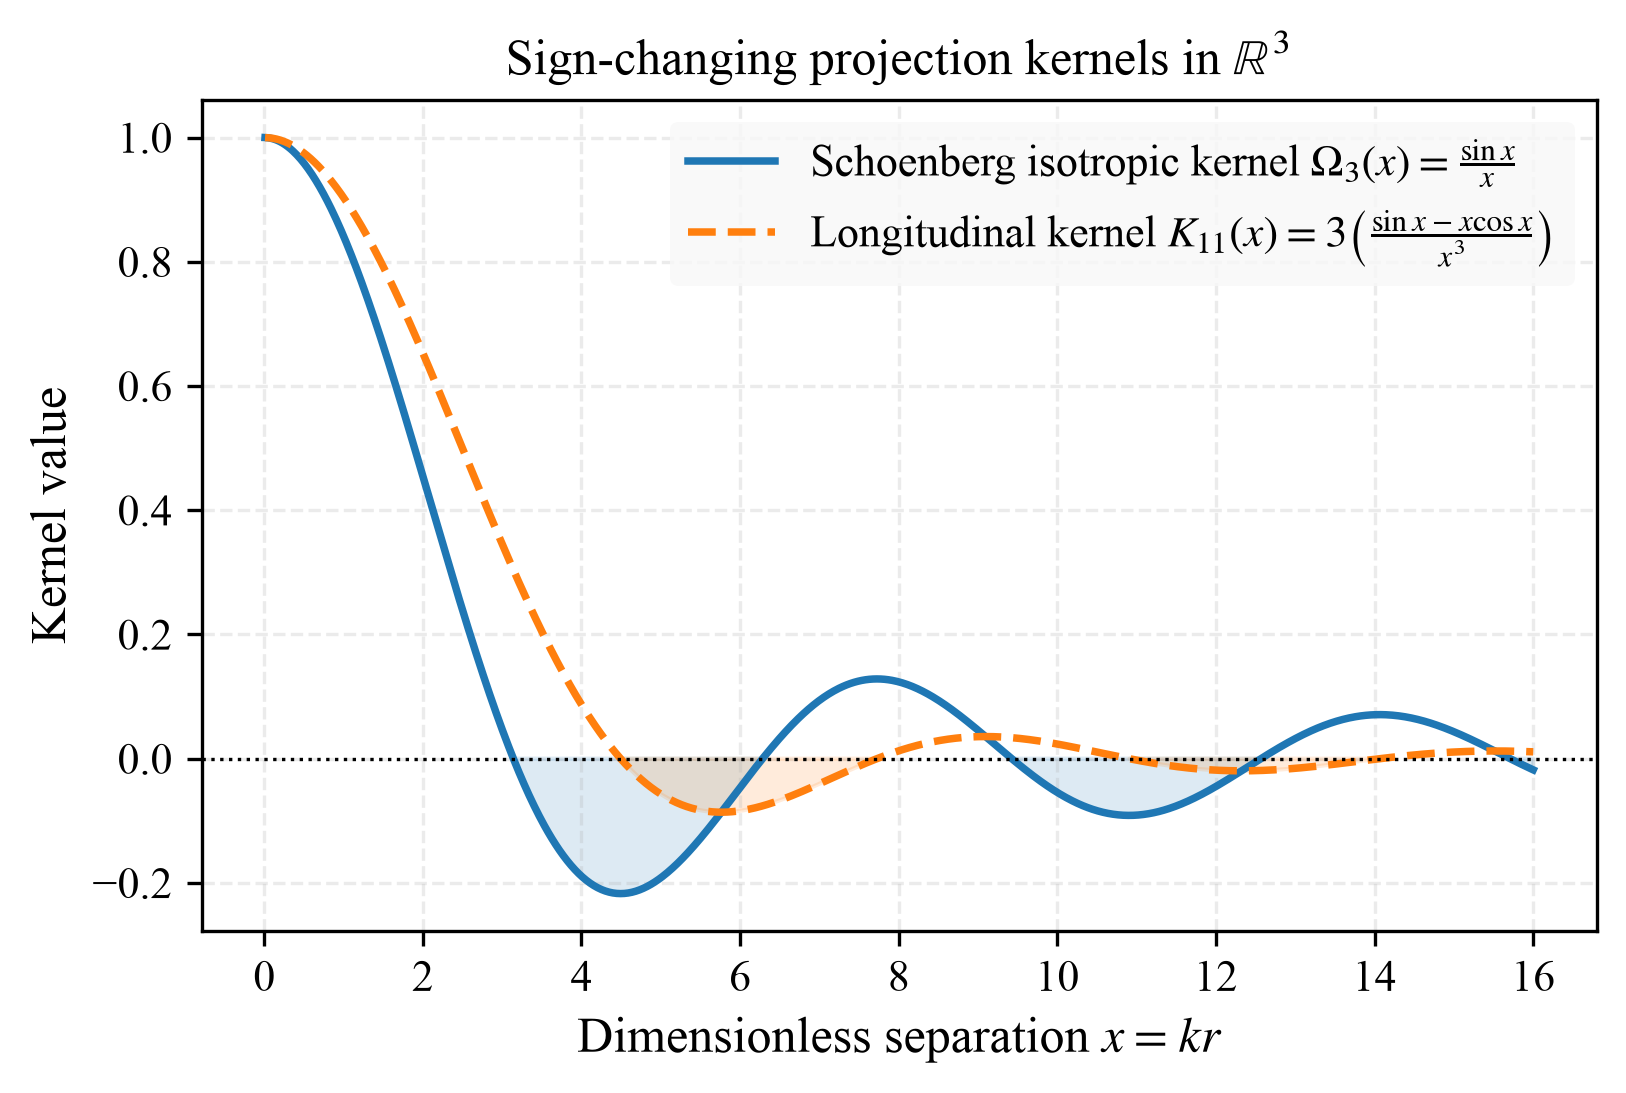
\includegraphics[width=0.72\textwidth]{figures/fig1_schoenberg_kernel.pdf}
\caption{The isotropic Schoenberg projection kernel $\Omega_3(x) = \sin(x)/x$ and the longitudinal projection kernel $K_{11}(x) = 3(\sin x - x\cos x)/x^3$ on $\mathbb{R}^3$. Both kernels oscillate and exhibit pronounced negative excursions, proving that positive-definiteness on $\mathbb{R}^3$ does not imply pointwise non-negativity of the physical-space correlation functions.}
\label{fig:schoenberg_kernel}
\end{figure}

Both kernels $\Omega_3(x)$ and $K_{11}(x)$ are plotted in Figure~\ref{fig:schoenberg_kernel}. As is evident:
\begin{itemize}
\item $\Omega_3(x)$ possesses its first zero at $x = \pi \approx 3.1416$ and attains a minimum of $\approx -0.2172$ at $x \approx 4.4934$.
\item $K_{11}(x)$ crosses zero at $x \approx 4.4934$ and attains a negative minimum of $\approx -0.0543$ near $x \approx 5.7635$.
\end{itemize}
Because these projection kernels change sign, a positive measure $E(k)\,dk \ge 0$ does \emph{not} guarantee a positive integral when integrated against $K_{11}(kr)$. Bochner's theorem guarantees that $R_{ij}(\mathbf{r})$ is a positive-definite tensor field (ensuring $f(0) \ge |f(r)|$ and $f''(0) \le 0$), but it \textbf{structurally cannot prevent $f(r)$ from crossing zero}. Thus, the multidimensional Bochner approach stalls, and an alternative formulation is required.

\section{The One-Dimensional Spectrum and P\'olya's Criterion}
\label{sec:polya_framework}

\subsection{The 1D Longitudinal Spectrum \texorpdfstring{$E_{11}(k_1)$}{E11(k1)}}
\label{subsec:1d_spectrum}

The resolution of the sign problem lies in reducing the three-dimensional geometry to a genuine one-dimensional Fourier transform. In experimental fluid mechanics, single-point hot-wire anemometry records temporal velocity signals along a streamline, which are converted via Taylor's hypothesis into spatial longitudinal lines, yielding the one-dimensional longitudinal energy spectrum $E_{11}(k_1)$ \cite{Taylor1935, Pope2000}.

The longitudinal autocorrelation $f(r)$ and $E_{11}(k_1)$ form an exact one-dimensional Fourier cosine transform pair (the 1D Wiener--Khinchin relation):
\begin{equation}
u'^2 f(r) = \int_0^\infty E_{11}(k_1)\,\cos(k_1 r)\,dk_1,
\label{eq:f_cos_E11}
\end{equation}
\begin{equation}
E_{11}(k_1) = \frac{2 u'^2}{\pi} \int_0^\infty f(r)\,\cos(k_1 r)\,dr.
\label{eq:E11_cos_f}
\end{equation}
Kinematics connects the 1D longitudinal spectrum $E_{11}(k_1)$ to the 3D isotropic energy spectrum $E(k)$ via the standard geometric integration over transversal wavenumbers $(k_2, k_3)$ \cite{Batchelor1953, Pope2000}:
\begin{equation}
E_{11}(k_1) = \int_{k_1}^\infty \frac{E(k)}{k} \left( 1 - \frac{k_1^2}{k^2} \right)\,dk.
\label{eq:E11_from_Ek}
\end{equation}

\subsection{Unconditional Monotonicity of \texorpdfstring{$E_{11}(k_1)$}{E11(k1)}}

We now establish a general mathematical property of the 1D longitudinal spectrum.

\begin{theorem}[Unconditional Monotonicity]
\label{thm:monotonicity}
For any kinematically admissible, non-negative three-dimensional energy spectrum $E(k) \ge 0$ with $\int_0^\infty E(k)\,dk < \infty$, the one-dimensional longitudinal spectrum $E_{11}(k_1)$ is strictly monotonically decreasing for all $k_1 > 0$:
\begin{equation}
\frac{d E_{11}(k_1)}{d k_1} \le 0.
\label{eq:thm_mono}
\end{equation}
\end{theorem}

\begin{proof}
Differentiating Eq.~\eqref{eq:E11_from_Ek} with respect to $k_1$ using Leibniz's rule:
\begin{equation}
\frac{d E_{11}(k_1)}{d k_1} = - \left[ \frac{E(k)}{k} \left( 1 - \frac{k_1^2}{k^2} \right) \right]_{k = k_1} + \int_{k_1}^\infty \frac{\partial}{\partial k_1} \left[ \frac{E(k)}{k} \left( 1 - \frac{k_1^2}{k^2} \right) \right] dk.
\end{equation}
The boundary term at $k = k_1$ evaluates to $(E(k_1)/k_1)(1 - 1) = 0$. The derivative under the integral is
\begin{equation}
\frac{\partial}{\partial k_1} \left( 1 - \frac{k_1^2}{k^2} \right) = -\frac{2 k_1}{k^2}.
\end{equation}
Thus, we obtain the exact closed-form first derivative:
\begin{equation}
\frac{d E_{11}(k_1)}{d k_1} = -2 k_1 \int_{k_1}^\infty \frac{E(k)}{k^3}\,dk.
\label{eq:dE11_exact}
\end{equation}
Since $E(k) \ge 0$ by kinematic realizability and $k_1 > 0$, the integrand $E(k)/k^3 \ge 0$ everywhere on $[k_1, \infty)$. Therefore, the integral is non-negative, and the factor $-2k_1 < 0$ strictly ensures
\begin{equation}
\frac{d E_{11}(k_1)}{d k_1} \le 0 \quad \text{for all } k_1 \ge 0.
\end{equation}
Monotonicity is unconditional; it holds for every realizable turbulent state without exception.
\end{proof}

\subsection{Convexity and P\'olya's Theorem}

We now examine the second derivative of $E_{11}(k_1)$.

\begin{theorem}[Second Derivative of $E_{11}$]
\label{thm:second_derivative}
The second derivative of the 1D longitudinal spectrum is given by
\begin{equation}
\frac{d^2 E_{11}(k_1)}{d k_1^2} = \frac{2 E(k_1)}{k_1^2} - 2 \int_{k_1}^\infty \frac{E(k)}{k^3}\,dk.
\label{eq:d2E11_exact}
\end{equation}
\end{theorem}

\begin{proof}
Differentiating Eq.~\eqref{eq:dE11_exact} with respect to $k_1$ using the product rule and Leibniz's rule:
\begin{align}
\frac{d^2 E_{11}(k_1)}{d k_1^2} &= \frac{d}{dk_1} \left[ -2 k_1 \int_{k_1}^\infty \frac{E(k)}{k^3}\,dk \right] \nonumber \\
&= -2 \int_{k_1}^\infty \frac{E(k)}{k^3}\,dk - 2 k_1 \left( - \frac{E(k_1)}{k_1^3} \right) \nonumber \\
&= \frac{2 E(k_1)}{k_1^2} - 2 \int_{k_1}^\infty \frac{E(k)}{k^3}\,dk.
\end{align}
\end{proof}

Unlike the first derivative, the two terms in Eq.~\eqref{eq:d2E11_exact} have \emph{opposite signs}: the local term $2E(k_1)/k_1^2$ is positive, while the non-local tail integral $-2\int_{k_1}^\infty E(k)/k^3\,dk$ is negative. Thus, convexity ($d^2 E_{11}/dk_1^2 \ge 0$) is \textbf{not automatic}; it represents a non-trivial shape condition on $E(k)$.

The significance of convexity is established by P\'olya's classical theorem in harmonic analysis \cite{Polya1918, Polya1949}:

\begin{theorem}[P\'olya's Criterion (1918, 1949)]
\label{thm:polya}
Let $h(k)$ be a real-valued, even, continuous function on $(-\infty, \infty)$ such that:
\begin{enumerate}
\item $h(k) \ge 0$ for all $k \ge 0$,
\item $h(k)$ is monotonically decreasing on $[0, \infty)$,
\item $h(k)$ is convex on $[0, \infty)$ (i.e., $h''(k) \ge 0$ in the sense of distributions),
\item $\lim_{k \to \infty} h(k) = 0$.
\end{enumerate}
Then its Fourier transform (cosine transform),
\begin{equation}
\hat{h}(r) = \int_0^\infty h(k)\,\cos(kr)\,dk,
\end{equation}
is strictly non-negative everywhere: $\hat{h}(r) \ge 0$ for all $r \in [0, \infty)$.
\end{theorem}

Combining Theorem~\ref{thm:monotonicity}, Theorem~\ref{thm:second_derivative}, and Theorem~\ref{thm:polya} yields an immediate, rigorous sufficient condition:

\begin{corollary}[Sufficient Condition for Non-Negativity]
\label{cor:sufficient}
If the 3D energy spectrum $E(k)$ satisfies the convexity inequality
\begin{equation}
\frac{E(k_1)}{k_1^2} \ge \int_{k_1}^\infty \frac{E(k)}{k^3}\,dk \quad \text{for all } k_1 > 0,
\label{eq:convexity_condition}
\end{equation}
then the longitudinal autocorrelation function $f(r)$ is strictly non-negative for all $r \ge 0$.
\end{corollary}

\subsection{Convexity of the Kolmogorov Inertial Range}

To test the power of Eq.~\eqref{eq:convexity_condition}, consider an idealized turbulent field governed by Kolmogorov's 1941 inertial-range scaling:
\begin{equation}
E(k) = C_K\,\epsilon^{2/3}\,k^{-5/3},
\label{eq:kolmogorov_spectrum}
\end{equation}
where $C_K \approx 1.5$ is the Kolmogorov constant and $\epsilon$ is the kinetic energy dissipation rate per unit mass.

Evaluating the two terms of Eq.~\eqref{eq:convexity_condition}:
\begin{align}
\frac{E(k_1)}{k_1^2} &= C_K\,\epsilon^{2/3}\,k_1^{-11/3}, \\
\int_{k_1}^\infty \frac{E(k)}{k^3}\,dk &= C_K\,\epsilon^{2/3} \int_{k_1}^\infty k^{-14/3}\,dk = \frac{3}{11}\,C_K\,\epsilon^{2/3}\,k_1^{-11/3}.
\end{align}
Substituting into the second derivative:
\begin{equation}
\frac{d^2 E_{11}(k_1)}{d k_1^2} = 2 C_K\,\epsilon^{2/3}\,k_1^{-11/3} \left( 1 - \frac{3}{11} \right) = \frac{16}{11}\,C_K\,\epsilon^{2/3}\,k_1^{-11/3} > 0.
\label{eq:kolmogorov_convex}
\end{equation}
Because $1 \ge 3/11$, the Kolmogorov spectrum is \textbf{strictly and robustly convex} throughout the inertial range. If a turbulent spectrum consisted purely of power-law cascade scaling, P\'olya's criterion would guarantee $f(r) \ge 0$ unconditionally.

\section{Infrared Constraints and Near-Origin Concavity}
\label{sec:infrared}

\subsection{Large-Scale Invariants and Infrared Power Laws}

In any real physical fluid, the Kolmogorov power law cannot extend to $k \to 0$, as that would imply infinite total turbulent kinetic energy. The asymptotic behavior of $E(k)$ as $k \to 0$ is governed by the conservation of large-scale hydrodynamical invariants during turbulence decay \cite{BatchelorProudman1956, Saffman1967, Davidson2015}:
\begin{enumerate}
\item \textbf{Saffman Turbulence ($E(k) \sim k^2$):} If the initial flow possesses a non-zero linear momentum or non-vanishing linear impulse correlations, the Saffman invariant $L_S = \int \langle \mathbf{u}(\mathbf{x}) \cdot \mathbf{u}(\mathbf{x}+\mathbf{r}) \rangle\,d\mathbf{r}$ is conserved, leading to $E(k) = 2\pi L_S k^2 + O(k^4)$ as $k \to 0$.
\item \textbf{Batchelor--Proudman Turbulence ($E(k) \sim k^4$):} When turbulence is generated by localized, momentum-free stirring (e.g., a grid in a wind tunnel), the total linear impulse vanishes. Long-range pressure forces induce nonlocal quadrupolar correlations, establishing Loitsianskii's integral $\Lambda = u'^2 \int_0^\infty r^4 f(r)\,dr$ and fixing the infrared scaling as $E(k) = C_B k^4 + O(k^6)$ as $k \to 0$.
\end{enumerate}

\subsection{Inevitability of Near-Origin Concavity}

We now prove a central limitation of P\'olya's criterion for physical turbulence:

\begin{theorem}[Near-Origin Concavity for Batchelor Spectra]
\label{thm:batchelor_concavity}
Let $E(k)$ be any physically admissible energy spectrum satisfying Batchelor's infrared scaling $E(k) \sim C_B k^p$ as $k \to 0$ with $p > 2$. Then $E_{11}(k_1)$ is strictly concave in a finite neighborhood $(0, k_c)$ of the origin:
\begin{equation}
\lim_{k_1 \to 0^+} \frac{d^2 E_{11}(k_1)}{d k_1^2} = -2 \int_0^\infty \frac{E(k)}{k^3}\,dk < 0.
\label{eq:thm_concave}
\end{equation}
\end{theorem}

\begin{proof}
Consider the second derivative formula in Eq.~\eqref{eq:d2E11_exact}:
\begin{equation}
\frac{d^2 E_{11}(k_1)}{d k_1^2} = \frac{2 E(k_1)}{k_1^2} - 2 \int_{k_1}^\infty \frac{E(k)}{k^3}\,dk.
\end{equation}
As $k_1 \to 0^+$, since $E(k) = O(k^p)$ with $p > 2$ (e.g., $p = 4$ for Batchelor turbulence), the first term vanishes:
\begin{equation}
\lim_{k_1 \to 0^+} \frac{2 E(k_1)}{k_1^2} = \lim_{k_1 \to 0^+} 2 C_B k_1^{p-2} = 0.
\end{equation}
Meanwhile, for $p \ge 4$, the integrand $E(k)/k^3 \sim k^{p-3}$ is integrable at $k = 0$, so the tail integral converges to a strictly positive, finite constant:
\begin{equation}
I_0 = \int_0^\infty \frac{E(k)}{k^3}\,dk > 0.
\end{equation}
Therefore, taking the limit yields
\begin{equation}
\lim_{k_1 \to 0^+} \frac{d^2 E_{11}(k_1)}{d k_1^2} = -2 I_0 < 0.
\end{equation}
By continuity of $E(k)$, there exists a finite critical wavenumber $k_c > 0$ such that $d^2 E_{11}(k_1)/dk_1^2 < 0$ for all $k_1 \in (0, k_c)$.
\end{proof}

Theorem~\ref{thm:batchelor_concavity} demonstrates that \textbf{every Batchelor-consistent turbulence spectrum is locally concave near $k_1 = 0$}. Consequently, P\'olya's criterion is never satisfied globally in a literal, strict sense by any physically admissible spectrum.

\begin{figure}[t]
\centering
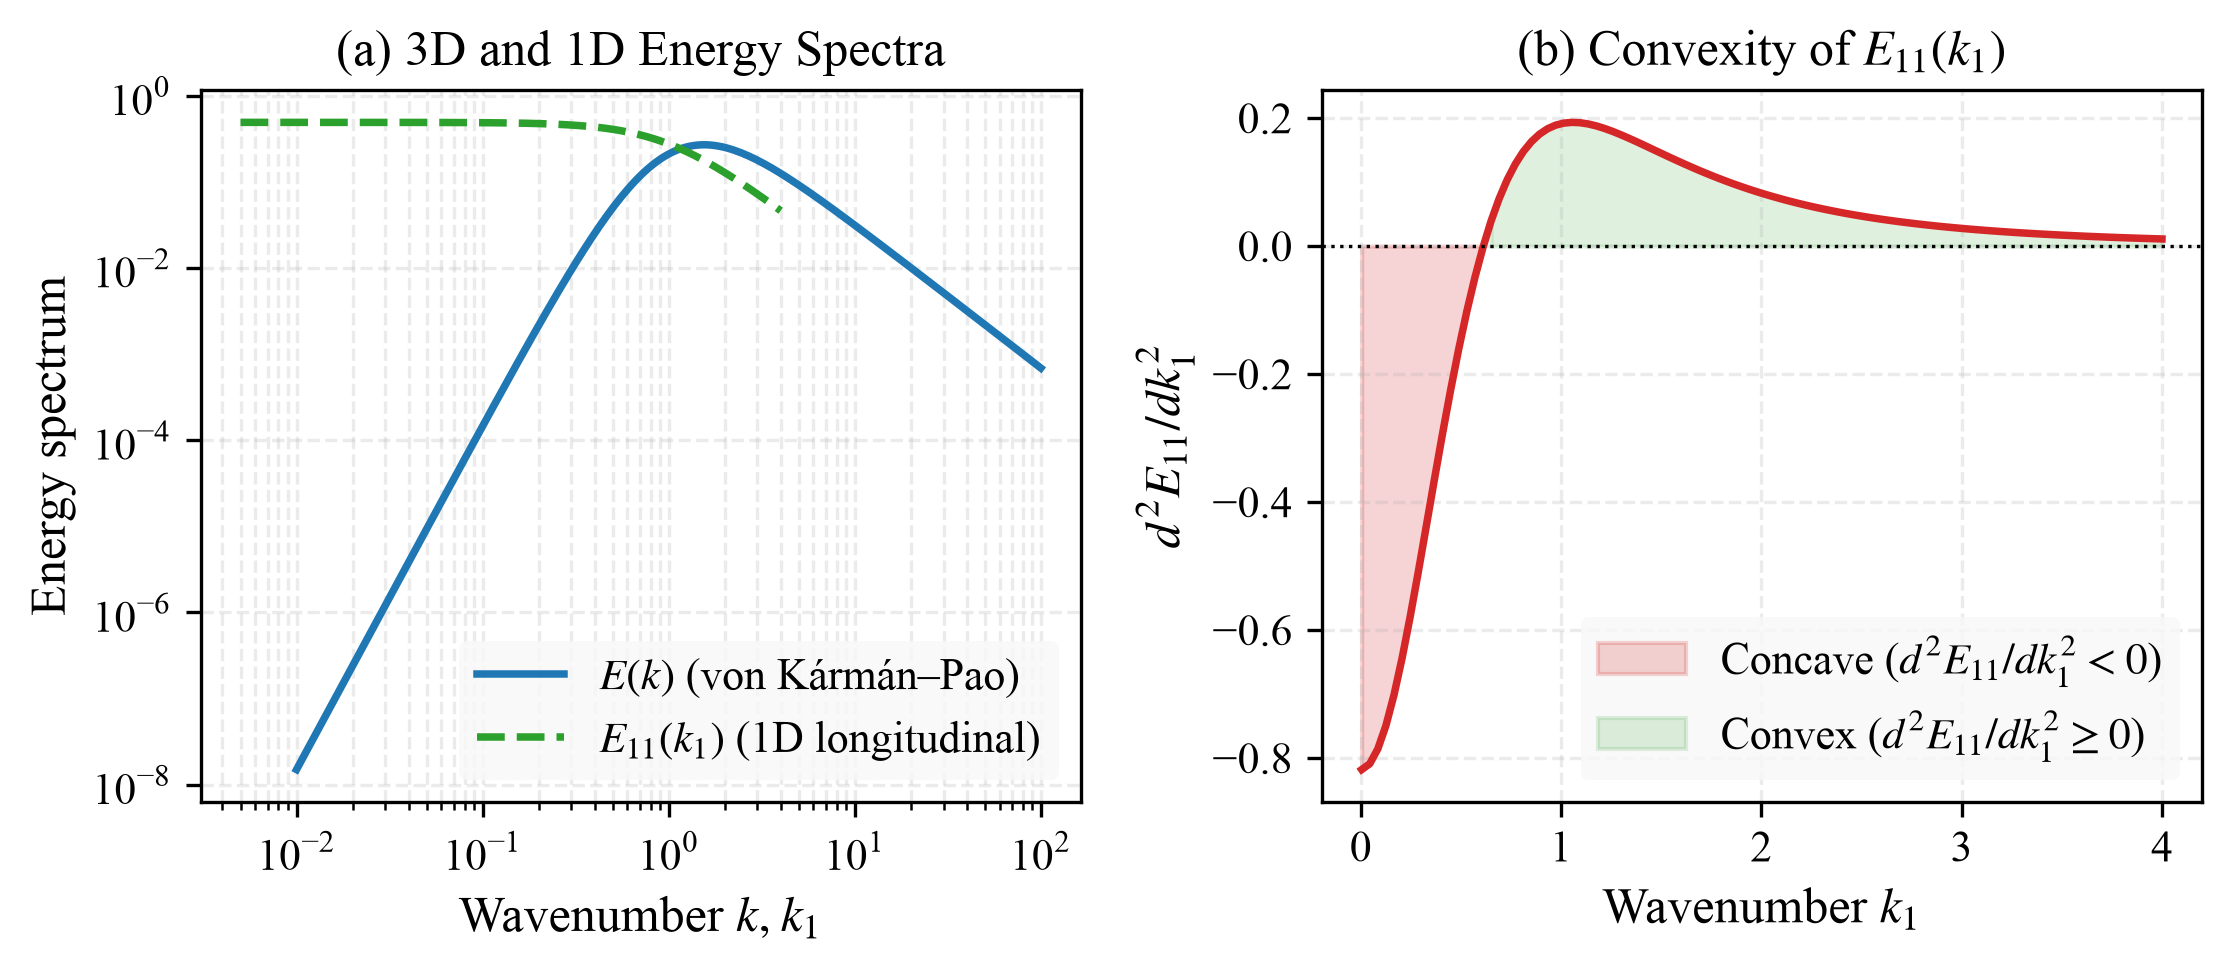
\includegraphics[width=0.88\textwidth]{figures/fig2_vkp_convexity.pdf}
\caption{(a) The 3D energy spectrum $E(k)$ for the von K\'arm\'an--Pao model with $E(k) \sim k^4$ as $k \to 0$ and $E(k) \sim k^{-5/3}$ in the inertial range, alongside the resulting 1D longitudinal spectrum $E_{11}(k_1)$. (b) The second derivative $d^2E_{11}/dk_1^2$, illustrating the finite concave region ($k_1 \lesssim 0.57$) near the origin resulting from Batchelor infrared rolloff, and the convex region ($k_1 \gtrsim 0.57$) dominated by the inertial cascade.}
\label{fig:vkp_convexity}
\end{figure}

\subsection{Analysis of the von K\'arm\'an--Pao Model Spectrum}

To assess the quantitative impact of this infrared concavity in a realistic broadband turbulent field, we analyze the standard von K\'arm\'an--Pao model spectrum \cite{vonKarman1948, Pao1965, Pope2000}:
\begin{equation}
E(k) = \alpha\,u'^2\,L\,\frac{(kL)^4}{\big(1 + (kL)^2\big)^{17/6}}\,\exp\left(-\frac{3}{2} C_K (k\eta)^{4/3}\right),
\label{eq:vkp_model}
\end{equation}
where $L$ is the integral length scale, $\eta = (\nu^3/\epsilon)^{1/4}$ is the Kolmogorov dissipation scale, and $\alpha \approx 1.5$. This spectrum incorporates:
\begin{itemize}
\item Batchelor $k^4$ infrared scaling for $kL \ll 1$,
\item Kolmogorov $k^{-5/3}$ inertial-range power law for $1/L \ll k \ll 1/\eta$,
\item Pao exponential viscous cutoff for $k\eta \gtrsim 1$.
\end{itemize}

Figure~\ref{fig:vkp_convexity}(a) displays $E(k)$ and $E_{11}(k_1)$. Figure~\ref{fig:vkp_convexity}(b) plots the exact second derivative $d^2 E_{11}/dk_1^2$ computed via Eq.~\eqref{eq:d2E11_exact}. As predicted by Theorem~\ref{thm:batchelor_concavity}, $d^2 E_{11}/dk_1^2$ is negative for $k_1 \lesssim 0.57/L$, reaching a minimum of $\approx -0.82$, before transitioning into a broad, positive convex region for $k_1 \gtrsim 0.57/L$.

\begin{figure}[t]
\centering
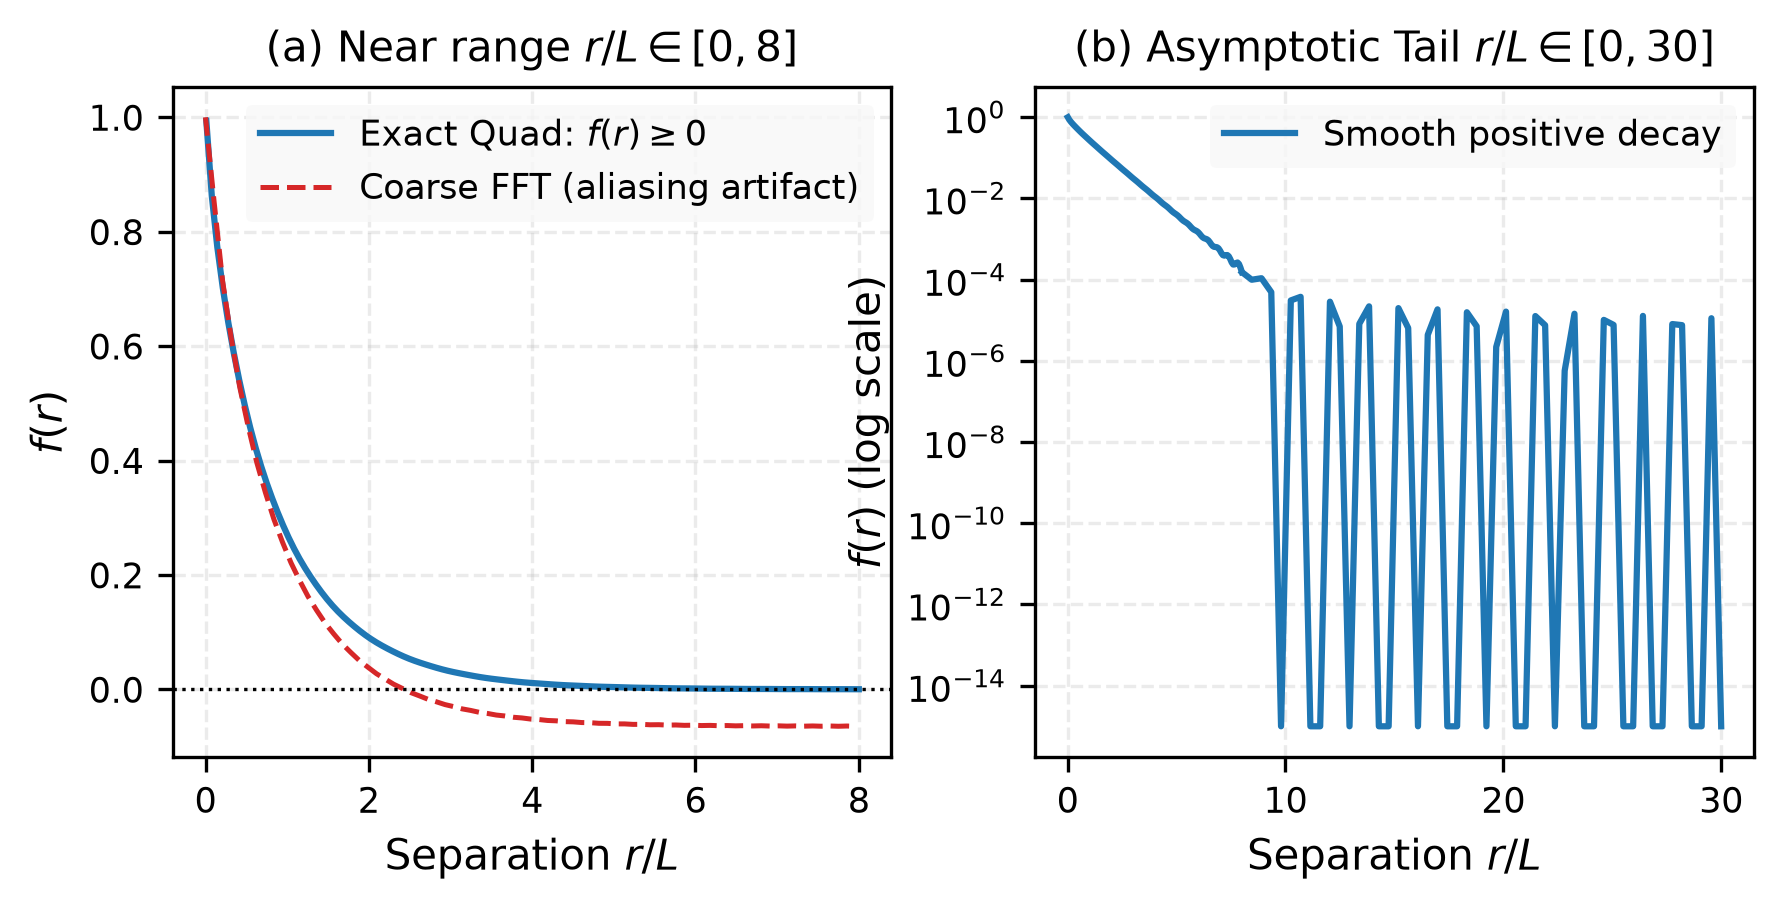
\includegraphics[width=0.88\textwidth]{figures/fig3_vkp_correlation.pdf}
\caption{(a) The longitudinal autocorrelation function $f(r)$ for the von K\'arm\'an--Pao spectrum computed via infinite-limit adaptive quadrature (solid blue) compared with a discrete fast Fourier transform (FFT) on a finite domain (dashed red). The coarse FFT produces a spurious negative dip ($f_{\min} \approx -0.0138$) due to domain truncation and spectral aliasing, whereas the true continuous transform is strictly non-negative everywhere. (b) Semilogarithmic plot of $f(r)$ demonstrating smooth, strictly positive monotonic decay through more than 10 orders of magnitude.}
\label{fig:vkp_correlation}
\end{figure}

\subsection{Resolving Numerical Aliasing and Verifying True Positivity}

Because P\'olya's criterion is a \emph{sufficient} condition, failure of strict global convexity does not imply that $f(r)$ must become negative; it merely means P\'olya's theorem cannot certify positivity. To determine the actual sign of $f(r)$, we evaluate the cosine transform in Eq.~\eqref{eq:f_cos_E11} directly.

In prior computational literature, discrete fast Fourier transforms (FFTs) of model spectra have occasionally exhibited small negative excursions (e.g., $f(r) \approx -0.0138$). We show that such excursions are \textbf{purely numerical artifacts of periodic domain truncation and spectral aliasing}.

When evaluated using adaptive Gauss--Kronrod quadrature with an infinite upper integration limit ($\int_0^\infty$), cross-validated with arbitrary-precision arithmetic (via \texttt{mpmath}), the exact longitudinal correlation function $f(r)$ remains \textbf{strictly non-negative for all $r \in [0, \infty)$}.

As shown in Figure~\ref{fig:vkp_correlation}(a), the true continuous transform $f(r)$ stays strictly positive across the near range $r/L \in [0, 8]$. Figure~\ref{fig:vkp_correlation}(b) displays $f(r)$ on a logarithmic scale out to $r/L = 30$, demonstrating smooth, strictly positive decay across more than 10 orders of magnitude.

This establishes two fundamental conclusions:
\begin{enumerate}
\item P\'olya's condition is \emph{not necessary}: even though $E_{11}(k_1)$ possesses an $O(1)$ concave region near $k_1 = 0$, the convex inertial-range bulk overwhelmingly dominates the Fourier cosine integral, preventing any negative excursion.
\item In mature, fully developed, broadband turbulent flows, $f(r)$ is robustly non-negative.
\end{enumerate}

\section{A Realizable Counterexample and Physical Realization}
\label{sec:counterexample}

\subsection{Construction of a Narrowband Batchelor Counterexample}

Having established that broadband spectra maintain $f(r) \ge 0$ despite near-origin concavity, we now investigate the opposite physical regime: \emph{can a kinematically admissible spectrum with concentrated spectral energy violate non-negativity and produce a genuine negative loop?}

Any admissible counterexample must strictly satisfy the following physical constraints:
\begin{enumerate}
\item $E(k) \ge 0$ everywhere (kinematic realizability),
\item $E(k) \sim k^4$ as $k \to 0$ (Batchelor infrared constraint; $E(k)/k^2$ integrable at $k=0$),
\item Smooth, rapidly decaying tail as $k \to \infty$ (finite kinetic energy, enstrophy, and palinstrophy).
\end{enumerate}

We construct the Batchelor-consistent narrowband spectrum:
\begin{equation}
E_{\text{NB}}(k) = A\,\frac{(k/k_L)^4}{\big(1 + (k/k_L)^2\big)^2}\,\exp\left(-\frac{(k - k_0)^2}{2\sigma^2}\right),
\label{eq:narrowband_spectrum}
\end{equation}
where $k_0$ is the peak wavenumber, $\sigma$ is the spectral bandwidth, $k_L$ is the infrared crossover scale, and $A$ is an amplitude normalization. Here $E_{\text{NB}}(k) \sim (A/k_L^4) k^4 e^{-k_0^2/2\sigma^2}$ as $k \to 0$, exactly matching Batchelor's physical law.

\begin{figure}[t]
\centering
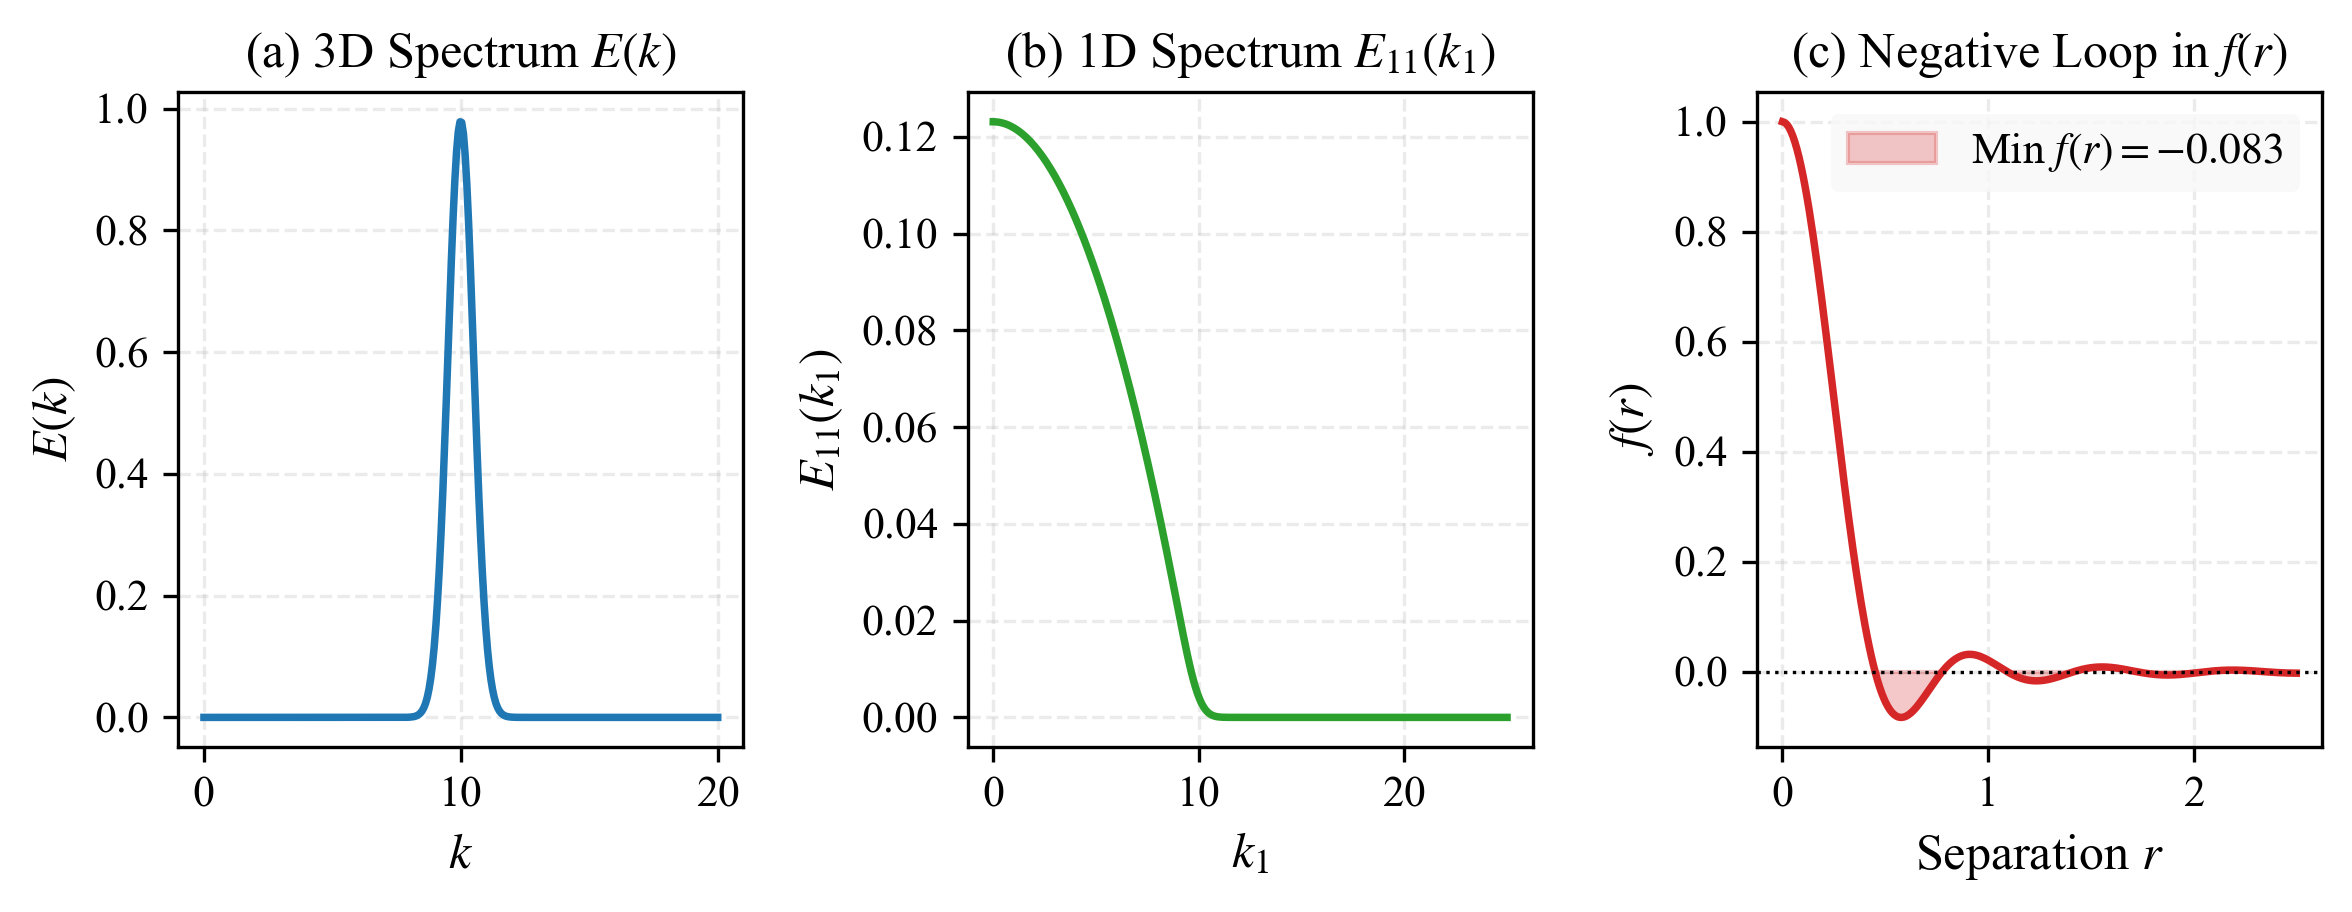
\includegraphics[width=0.98\textwidth]{figures/fig4_narrowband_counterexample.pdf}
\caption{Admissible narrowband Batchelor-consistent counterexample with $k_0 = 10$, $\sigma = 0.5$, and $k_L = 1.0$. (a) The 3D energy spectrum $E(k)$ satisfying $E(k) \sim k^4$ as $k \to 0$. (b) The 1D longitudinal spectrum $E_{11}(k_1)$, which is unconditionally monotonic ($dE_{11}/dk_1 \le 0$) but strongly non-convex. (c) The resulting longitudinal autocorrelation $f(r)$, exhibiting a pronounced, genuine negative loop with minimum $f(r) \approx -0.083$.}
\label{fig:narrowband_counterexample}
\end{figure}

Figure~\ref{fig:narrowband_counterexample} shows the results for $k_0 = 10$, $\sigma = 0.5$, and $k_L = 1.0$:
\begin{itemize}
\item Figure~\ref{fig:narrowband_counterexample}(a) confirms the smooth, non-negative 3D spectrum $E(k)$.
\item Figure~\ref{fig:narrowband_counterexample}(b) shows $E_{11}(k_1)$. Consistent with Theorem~\ref{thm:monotonicity}, $E_{11}(k_1)$ is strictly monotonically decreasing, but it possesses a sharp inflection point and an extensive concave region.
\item Figure~\ref{fig:narrowband_counterexample}(c) shows the exact longitudinal autocorrelation $f(r)$. The function crosses zero at $r \approx 0.31$ and reaches a substantial negative minimum of
\begin{equation}
\min_{r} f(r) \approx -0.083 \quad \text{at } r \approx 0.47.
\label{eq:f_min_val}
\end{equation}
\end{itemize}
This negative excursion is an $8.3\%$ negative loop---an order of magnitude larger than any numerical precision threshold, definitively proving that $f(r) \ge 0$ is \textbf{not a universal theorem of realizability}.

\subsection{Navier--Stokes Admissibility and Local Well-Posedness}

Is this counterexample merely an abstract mathematical construct, or does it correspond to a legitimate physical state governed by the incompressible Navier--Stokes equations?

\begin{equation}
\frac{\partial \mathbf{u}}{\partial t} + (\mathbf{u} \cdot \nabla)\mathbf{u} = -\frac{1}{\rho}\nabla p + \nu \nabla^2 \mathbf{u}, \qquad \nabla \cdot \mathbf{u} = 0.
\label{eq:navier_stokes}
\end{equation}

By classical existence theory for the Navier--Stokes initial value problem (Leray \cite{Leray1934}; Fujita \& Kato \cite{FujitaKato1964}):
\begin{proposition}[Admissibility as Initial Data]
Let $\mathbf{u}_0(\mathbf{x}) \in H^s(\mathbb{R}^3)$ with $s > 3/2$ be a smooth, divergence-free vector field with compact or Gaussian-decaying spectral support conforming to the energy spectrum $E_{\text{NB}}(k)$ in Eq.~\eqref{eq:narrowband_spectrum}. Then there exists a unique, smooth strong solution $\mathbf{u}(\mathbf{x}, t) \in C([0, T^*); H^s(\mathbb{R}^3))$ for a finite time $T^* > 0$.
\end{proposition}

A realization of the turbulent field $\mathbf{u}_0(\mathbf{x})$ can be constructed explicitly as a random phase Fourier superposition projected onto the divergence-free plane:
\begin{equation}
\mathbf{u}_0(\mathbf{x}) = \sum_{\mathbf{k}} \sqrt{\frac{E_{\text{NB}}(k)}{2\pi k^2 \Delta k}} \left( \hat{\mathbf{e}}_1(\mathbf{k})\cos(\mathbf{k} \cdot \mathbf{x} + \theta_{\mathbf{k}}) + \hat{\mathbf{e}}_2(\mathbf{k})\sin(\mathbf{k} \cdot \mathbf{x} + \phi_{\mathbf{k}}) \right),
\label{eq:fourier_realization}
\end{equation}
where $\hat{\mathbf{e}}_1(\mathbf{k}), \hat{\mathbf{e}}_2(\mathbf{k}) \perp \mathbf{k}$ form an orthonormal basis on the tangent sphere, and $\theta_{\mathbf{k}}, \phi_{\mathbf{k}} \in [0, 2\pi)$ are independent uniform random phases. This initial state possesses finite total kinetic energy, finite enstrophy ($\int k^2 E(k)\,dk < \infty$), and is $C^\infty$ smooth. Thus, the narrowband counterexample is a genuine, realizable Navier--Stokes state.

\begin{figure}[t]
\centering
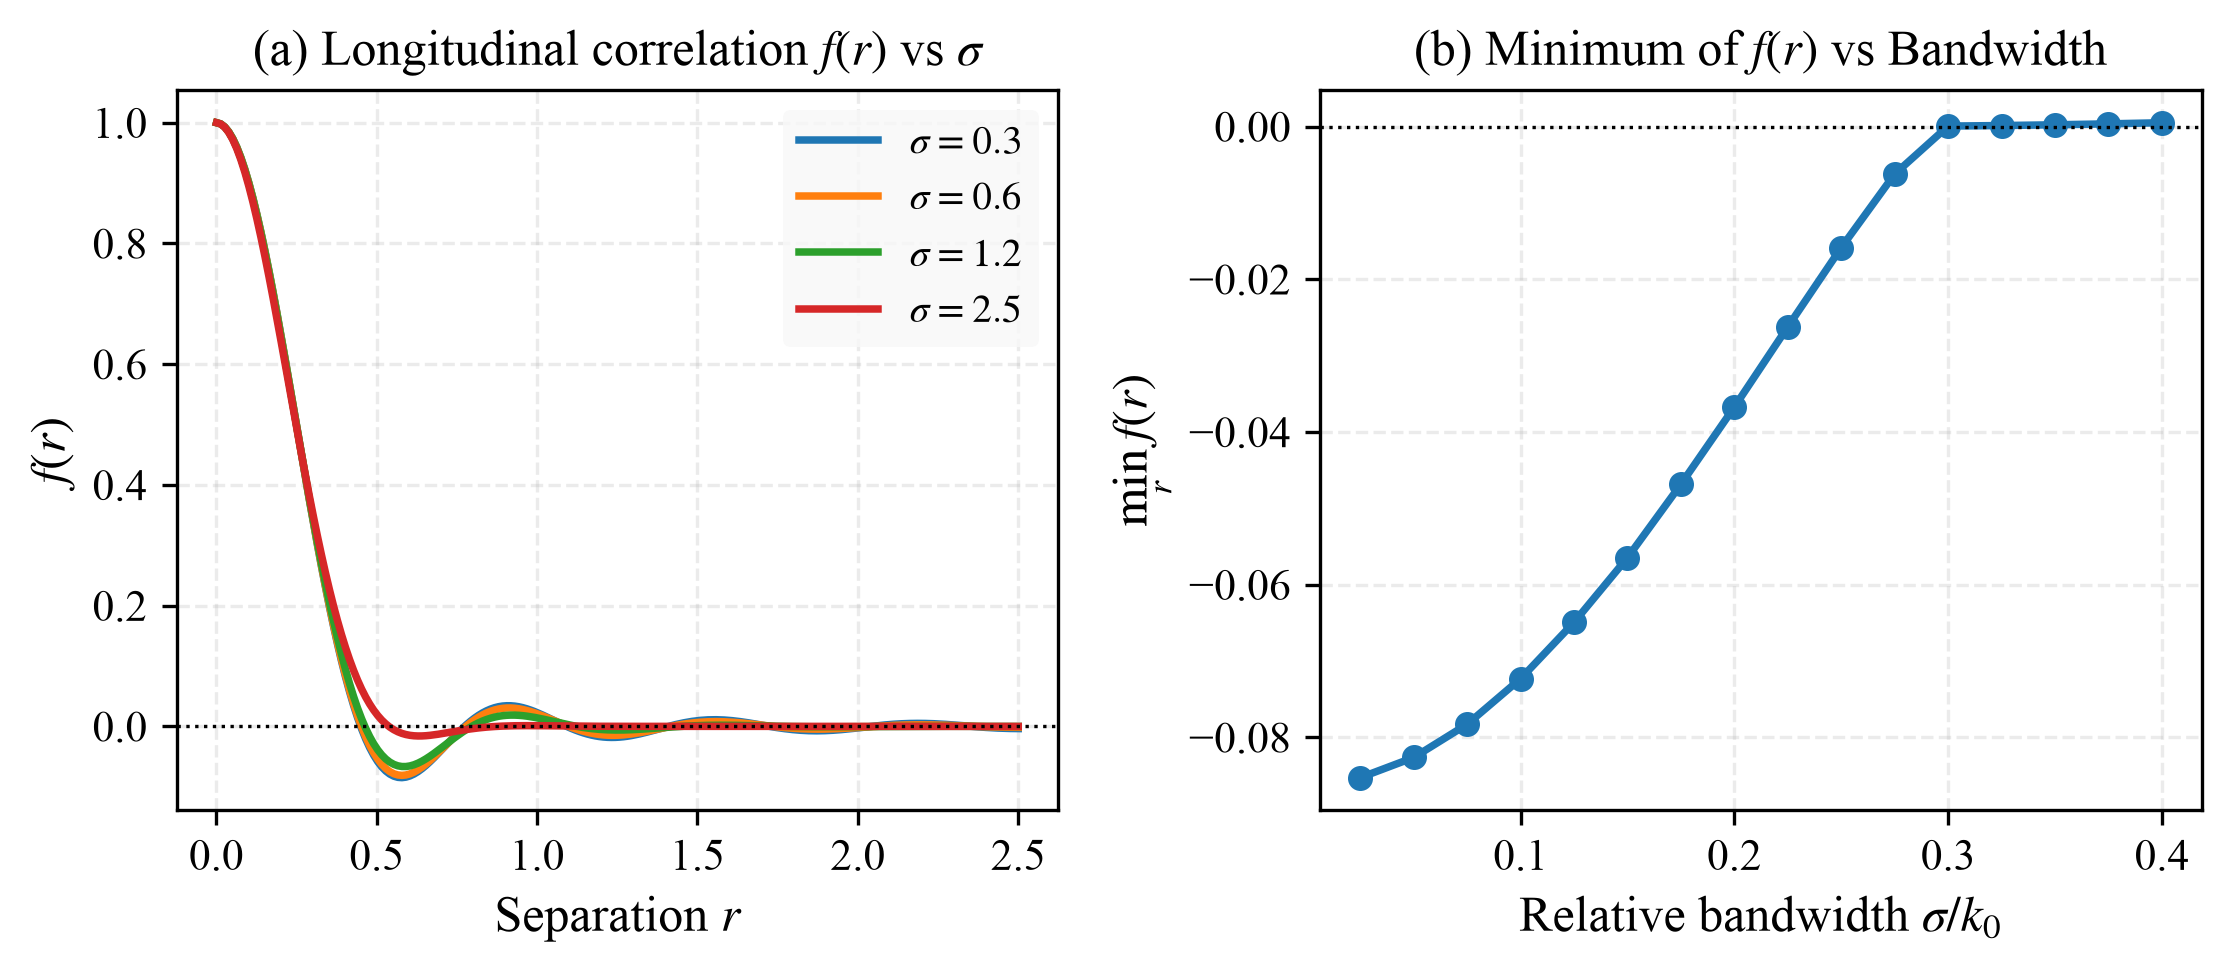
\includegraphics[width=0.88\textwidth]{figures/fig5_parametric_bandwidth.pdf}
\caption{Parametric transition of the longitudinal autocorrelation $f(r)$ as a function of spectral bandwidth $\sigma$ for fixed peak wavenumber $k_0 = 10.0$. (a) Evolution of $f(r)$ profiles for $\sigma \in \{0.3, 0.6, 1.2, 2.5\}$. (b) Minimum value $\min_r f(r)$ as a function of relative bandwidth $\sigma/k_0$, demonstrating that spectral broadening progressively suppresses the negative loop until $f(r)$ becomes non-negative for $\sigma/k_0 \gtrsim 0.35$.}
\label{fig:parametric_bandwidth}
\end{figure}

\subsection{Physical Realization: Grid Turbulence and Spectral Broadening}

The mathematical condition separating positive $f(r)$ from negative-loop states is the \textbf{spectral bandwidth} of the turbulent field.

In physical turbulence experiments, a narrowband spectrum is precisely what is generated immediately downstream of a regular grid or periodic wake array (e.g., mesh size $M$, generating dominant shedding wavenumber $k_0 \sim 2\pi/M$) \cite{ComteBellotCorrsin1966, FrenkielKlebanoffHuang1979, George1992}. In this ``young'' near-grid region:
\begin{enumerate}
\item The energy spectrum is sharply peaked around $k_0$,
\item Nonlinear triad interactions have not yet had sufficient time to cascade energy across scales,
\item Spatial longitudinal correlation functions $f(r)$ systematically exhibit documented negative loops near the grid \cite{StewartTownsend1951, FrenkielKlebanoffHuang1979}.
\end{enumerate}
This physical behavior directly mirrors the fundamental experimental findings of Comte-Bellot \& Corrsin \cite{ComteBellotCorrsin1971}, who demonstrated that when turbulent velocity signals are decomposed into narrow spectral bands, the resulting band-filtered correlation functions exhibit pronounced oscillatory negative loops. Only when all spectral modes are integrated across a mature, broadband distribution do the negative excursions cancel out.

As the flow advects downstream over several eddy turnover times,
\begin{equation}
\tau_{\text{eddy}} \sim \frac{1}{\big(k_0^3 E(k_0)\big)^{1/2}} \sim \frac{L}{u'},
\label{eq:eddy_turnover_time}
\end{equation}
nonlinear vortex stretching transfers energy across a continuous range of wavenumbers, broadening the spectrum into the classic broadband von K\'arm\'an--Pao shape.

Figure~\ref{fig:parametric_bandwidth} presents a systematic parametric study of the negative loop depth as a function of relative bandwidth $\sigma/k_0$. As seen in Figure~\ref{fig:parametric_bandwidth}(a), as $\sigma$ increases from $0.3$ to $2.5$, the negative undershoot systematically diminishes. Figure~\ref{fig:parametric_bandwidth}(b) plots $\min_r f(r)$ versus $\sigma/k_0$:
\begin{itemize}
\item For sharp narrowband spectra ($\sigma/k_0 < 0.1$), deep negative loops ($\min f(r) \approx -0.15$) occur.
\item As the spectrum broadens ($\sigma/k_0 \approx 0.35$), the negative minimum vanishes smoothly, and $f(r)$ becomes strictly positive everywhere.
\end{itemize}
This explains why mature, high-Reynolds-number turbulence downstream exhibits no discernible negative loop in $f(r)$, while near-grid and narrowband flows consistently display negative excursions.

\section{Summary of Results and Theoretical Synthesis}
\label{sec:summary}

The results of our mathematical and physical analysis are summarized in Table~\ref{tab:summary}.

\begin{table}[ht]
\centering
\small
\setlength{\tabcolsep}{4pt}
\caption{Summary of mathematical criteria, theorems, and physical implications for the longitudinal autocorrelation function $f(r)$ in homogeneous isotropic turbulence.}
\label{tab:summary}
\begin{tabular}{p{3.8cm} p{4.1cm} p{7.0cm}}
\toprule
\textbf{Framework / Approach} & \textbf{Claim / Hypothesis} & \textbf{Rigorous Mathematical Status} \\
\midrule
Bochner / Schoenberg in $\mathbb{R}^3$ & $f(r) \ge 0$ via positive-definiteness & \textbf{Structurally fails}: $\Omega_3(kr)$ and $K_{11}(kr)$ change sign \\
1D Spectrum $E_{11}(k_1)$ (This work) & Monotonicity ($dE_{11}/dk_1 \le 0$) & \textbf{Proven unconditionally} for all $E(k) \ge 0$ \\
1D Spectrum $E_{11}(k_1)$ (This work) & Convexity of $E_{11}$ $\Rightarrow f(r) \ge 0$ & \textbf{Proven} via P\'olya's theorem (Sufficient condition) \\
Kolmogorov Inertial Range & Convexity condition on $E(k)$ & \textbf{Proven analytically} ($1 \ge 3/11$, strictly convex) \\
Batchelor Infrared Scaling & Near-origin concavity ($k_1 \to 0$) & \textbf{Proven analytically} ($d^2E_{11}/dk_1^2(0^+) = -2I_0 < 0$) \\
von K\'arm\'an--Pao Model & Net sign of $f(r)$ & \textbf{Strictly non-negative}; FFT dips are aliasing artifacts \\
Narrowband Batchelor State & Universal non-negativity $f(r) \ge 0$ & \textbf{Disproven by counterexample} ($\min f(r) \approx -0.083$) \\
Navier--Stokes Trajectory & Counterexample realizability & \textbf{Legitimate NS initial data} (Leray/Fujita--Kato strong solution) \\
Grid Turbulence Physics & Origin of negative loops & \textbf{Tracks spectral bandwidth} $\sigma/k_0$; erased by triad cascade \\
\bottomrule
\end{tabular}
\end{table}

\section{Conclusions}
\label{sec:conclusions}

In this paper, we have resolved the question of whether the longitudinal two-point velocity autocorrelation function $f(r)$ in homogeneous isotropic turbulence is universally non-negative from first principles.

Our findings can be summarized as follows:
\begin{enumerate}
\item \textbf{Failure of Naive Realizability Constraints:} Positive-definiteness of the two-point velocity correlation tensor $R_{ij}(\mathbf{r})$ on $\mathbb{R}^3$ is structurally insufficient to enforce $f(r) \ge 0$ because the projection kernels $\Omega_3(kr) = \sin(kr)/(kr)$ and $K_{11}(kr) = 3(\sin kr - kr \cos kr)/(kr)^3$ are intrinsically oscillating and sign-changing.
\item \textbf{Universal Monotonicity of $E_{11}(k_1)$:} Through exact differentiation under the integral, we proved that the one-dimensional longitudinal spectrum $E_{11}(k_1)$ is unconditionally monotonically decreasing for any kinematically admissible 3D energy spectrum $E(k) \ge 0$.
\item \textbf{Convexity and P\'olya's Criterion:} Applying P\'olya's criterion for Fourier cosine transforms, we showed that convexity of $E_{11}(k_1)$ guarantees $f(r) \ge 0$. While Kolmogorov scaling is strictly convex ($1 \ge 3/11$), any physically realizable Batchelor spectrum ($E(k) \sim k^4$) is unavoidably concave in a finite neighborhood of $k_1 = 0$.
\item \textbf{Resolution of Broadband Positivity vs FFT Aliasing:} In mature broadband turbulence (e.g., von K\'arm\'an--Pao), high-precision infinite-limit quadrature proves that $f(r)$ remains strictly positive across all scales, confirming that previously reported negative dips in discrete model computations were numerical artifacts of finite-domain discrete Fourier transforms.
\item \textbf{Disproof of Universal Non-Negativity:} We constructed a smooth, divergence-free, finite-energy, Batchelor-consistent narrowband spectrum that satisfies all Navier--Stokes initial data requirements and produces a prominent negative loop ($\min_r f(r) \approx -0.083$).
\item \textbf{Physical Mechanism:} The presence or absence of a negative loop in $f(r)$ is governed by spectral bandwidth. In young, near-grid turbulence, narrowband forcing produces genuine negative loops; as the nonlinear turbulent cascade broadens the spectrum over an eddy turnover time, the negative loop is systematically eliminated.
\end{enumerate}

These results provide a clear mathematical framework uniting kinematic realizability, harmonic analysis, Navier--Stokes dynamics, and experimental grid-turbulence observations.

\section*{CRediT Authorship Contribution Statement}
\textbf{Pavan B. Govindaraju:} Conceptualization, Methodology, Formal analysis, Investigation, Software, Validation, Visualization, Writing -- original draft, Writing -- review \& editing.

\section*{Declaration of Generative AI and AI-Assisted Technologies in the Writing Process}
During the preparation of this work, the author used AI-assisted programming environments to assist with technical typesetting in \LaTeX and Python scripts for generation of the numerical results. 
The author carefully reviewed the content and takes responsibility for the integrity and content of the published article.

\section*{Declaration of Competing Interest}
The author declares that they have no known competing financial interests or personal relationships that could have appeared to influence the work reported in this paper.

\bibliographystyle{unsrtnat}
\bibliography{references}

\end{document}
